\subsection{Introducción}\label{header-n3}

La energía procedente del mar es un recurso que presenta en la
actualidad muchos retos tecnológicos y sociales a superar.
Principalmente, su desarrollo depende de un apoyo institucional en
inversiones I+D+I, que permita el estudio de un prototipo, teniendo las
infraestructuras necesarias para ensayar y demostrar su funcionamiento,
hasta llegar a la explotación comercial.

En este apartado se tratará de ofrecer una perspectiva general de las
diferentes fuentes de obtención disponibles en el océano, y junto con
ello, algunos de los mecanismos utilizados para la extracción de
energía.

\subsection{Tipos de infraestructura}\label{header-n8}

Existen diferentes
\href{http://www.udc.es/iuem/documentos/doc_xornadas/anaeco/APROVEITAMENTODAENERXIADASOLAS.pdf}{tipos
de infraestructuras} que permiten estudiar los sistemas de captación de
energía antes de su explotación comercial:

\textbf{Canales de pruebas:} Utilizados para analizar el comportamiento
hidrodinámico de prototipos iniciales a pequeña escala y validar su
diseño conceptual.

\textbf{Infraestructuras de test:} Prototipos a escala 1/10 o 1/3, en
esta fase, las pruebas se realizan en el medio marino, en zonas
protegidas, con oleaje restringido y de fácil acceso.

\textbf{Infraestructuras de demostración:} Prototipos pre-comerciales,
probados en mar abierto y conectados a la red eléctrica, para su
demostración y operación.

Algunos de los laboratorios de experimentación marítima son:

\begin{itemize}
\item
  El Centro de Estudios y Experimentación de Obras Públicas,
  \href{http://www.cedex.es/CEDEX/LANG_CASTELLANO/ORGANISMO/CENTYLAB/}{CEDEX},
  en Madrid, se estructura en varios órganos especializados en
  diferentes materias, entre ellos están el Centro de Estudios
  Hidrográficos (CEH) y el Centro de Estudios de Puertos y Costas
  (CEPYC). El primero, se centra en temas de planificación hidráulica,
  hidrología, ingeniería de las aguas continentales, así como en los
  aspectos relacionados con la calidad del recurso. Por otro lado, el
  CEPYC, está especializado en tareas de asistencia técnica,
  investigación y desarrollo tecnológico e innovación en materia de
  transporte.

  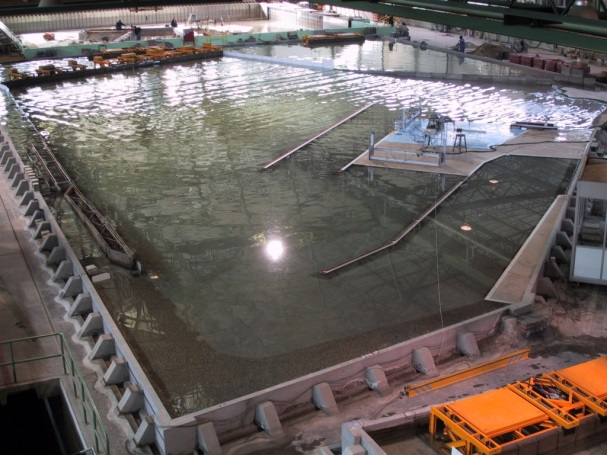
\includegraphics{/home/lewi/geaWaves/gea-waves/_hugo/content/tfg/1MEMORIA/imgMemoria/51-CEPYC.jpg}

  \textbf{Figura 5.1}: Fotografía del laboratorio
  \href{http://www.cedex.es/CEDEX/LANG_CASTELLANO/ORGANISMO/CENTYLAB/CEPYC/EQUIPAMIENTO/LEM0.htm}{CEPYC}
\end{itemize}

\begin{itemize}
\item
  El Laboratorio de Dinámica de Flujos Ambientales, en la Universidad de
  Granada (UGR), consta de cuatro instalaciones principales, dos
  situadas en CEAMA, y las otras dos en la ETS de Ingenieros de Caminos,
  Canales y Puertos. Entre ellas, se puede encontrar un Canal de
  Generación de Ola-Corriente, un Tanque de Oleaje Multidireccional, un
  Canal Basculante y un Tanque de difusión. Así mismo, desde el 2002,
  trabajan con sistemas de monitorización costera, habiendo realizado
  instalaciones en el Faro de Sacratif (Carchuna, Granada), Faro de
  Trafalgar (Cádiz), desembocadura del río San Pedro (Cádiz) y
  desembocadura del río Guadalquivir. La finalidad, reside en el control
  ambiental, estudios de parámetros morfodinámicos, gestión integral de
  zonas costeras, entre otras.

  \begin{figure}
  \centering
  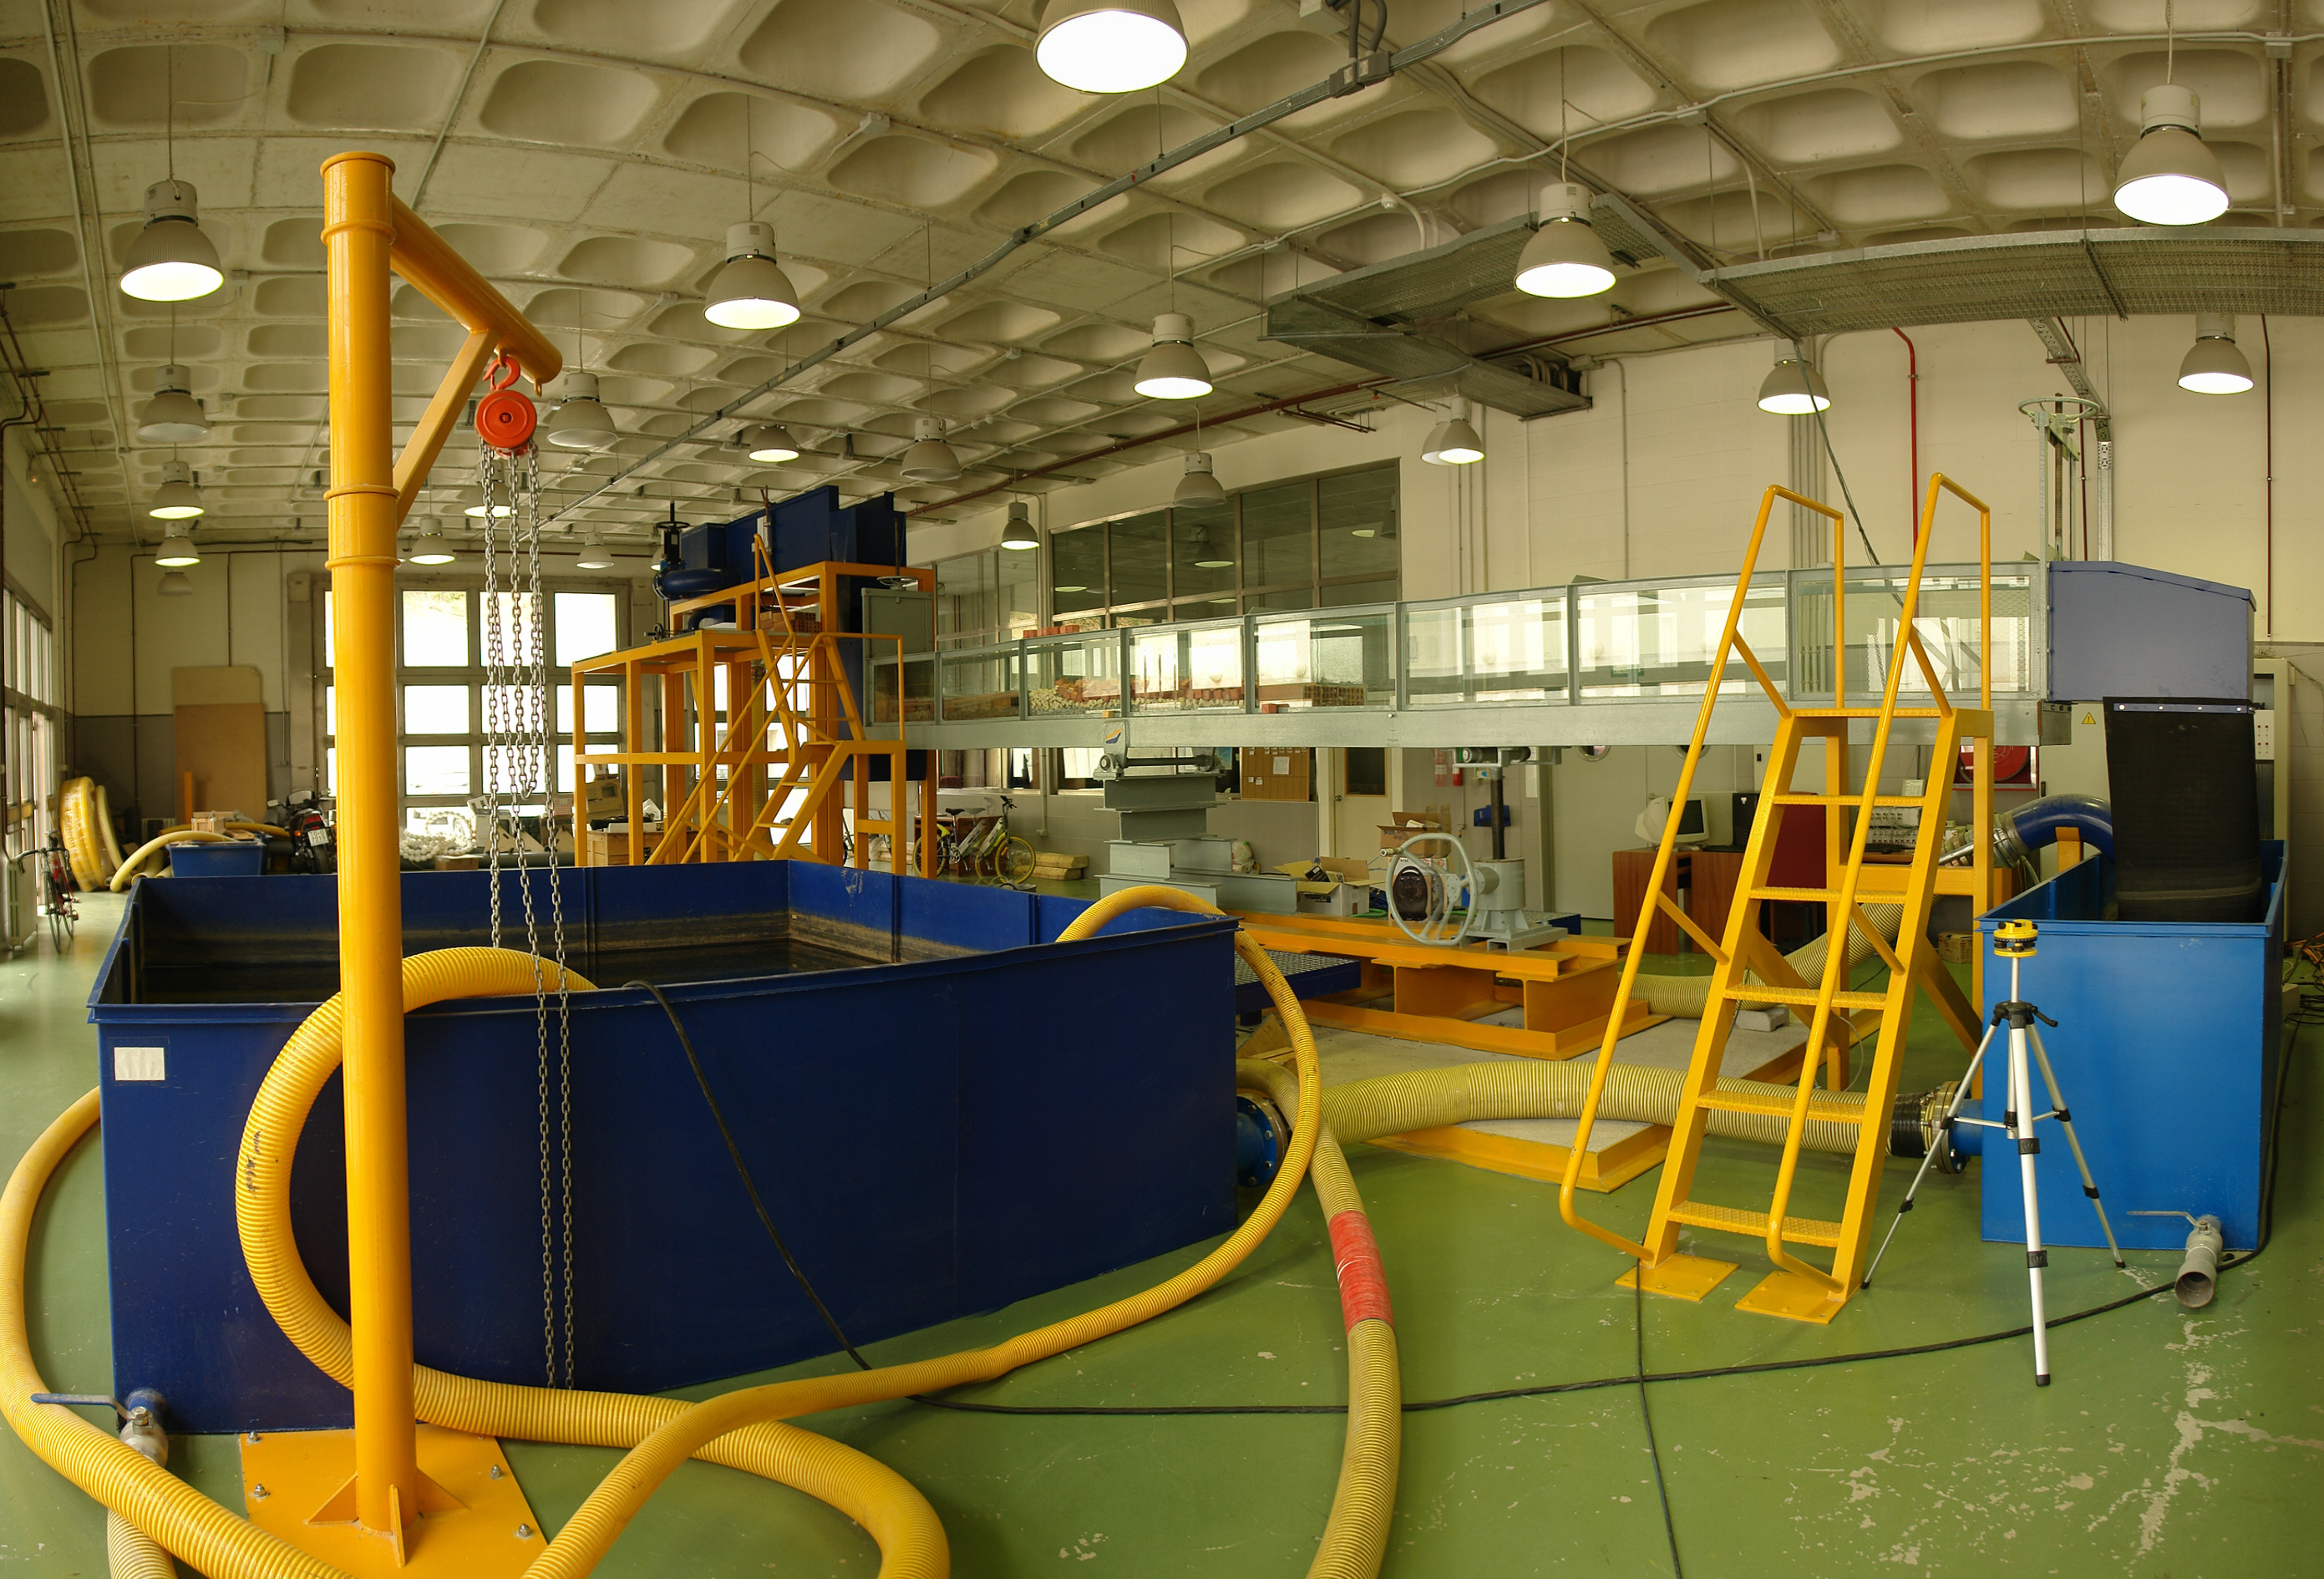
\includegraphics{/home/lewi/geaWaves/gea-waves/_hugo/content/tfg/1MEMORIA/imgMemoria/52-UGR.jpg}
  \caption{}
  \end{figure}
\end{itemize}

También existen empresas como
\href{https://www.boschrexroth.com/es/mx/industrias/aplicaciones-e-ingenieria-de-maquinaria/investigacion-hidrodinamica/hydrodynamic-research-1}{Boch
Rexroth}, que ofrecen soluciones de sistemas para laboratorios de
investigación hidrodinámica. Ante las diferentes condiciones como el
viento, las corrientes, la profundidad del agua y las temperaturas, que
influyen en el oleaje, se dedican a la generación controlada de olas.
Dando lugar a sistemas personalizados de accionamiento y control para
generadores y absorbedores de olas, así como fijaciones para piscinas
con suelo móvil ajustable. Además, suministran programas de cálculo y
análisis y recogida de datos.\\

\begin{figure}
\centering
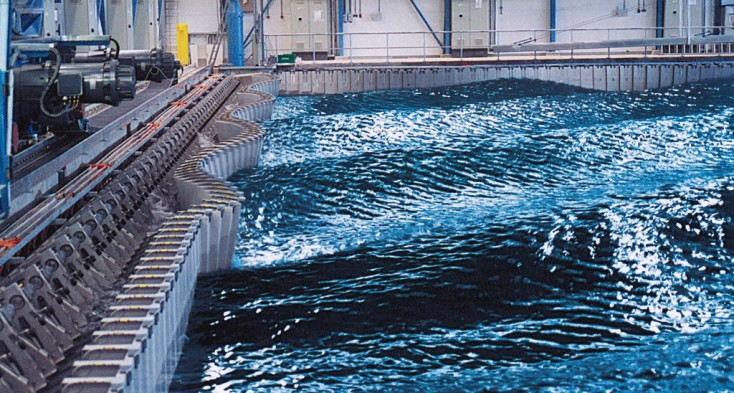
\includegraphics{/home/lewi/geaWaves/gea-waves/_hugo/content/tfg/1MEMORIA/imgMemoria/53-bochrexroth.jpg}
\caption{}
\end{figure}

Figura 5.3: Laboratorio de investigación
{[}\url{https://www.boschrexroth.com/es/mx/industrias/aplicaciones-e-ingenieria-de-maquinaria/investigacion-hidrodinamica/hydrodynamic-research-1}{]}

Se han patentado prototipos de todo tipo que utilizan diferentes
técnicas para la captación de energía de las olas. Aun así, pocas son
las instalaciones que se han ensayado en el mar a escala natural, por lo
que falta experiencia operativa con prototipos.

\subsection{Clasificación de sistemas de captación}\label{header-n44}

Los diseños de los captadores difieren entre sí, sobre todo, por el
origen de la energía que son capaces de aprovechar, así hasta el momento
se han estudiado formas para la extracción de:

\begin{itemize}
\item
  \textbf{La energía de las mareas o mareomotriz}: Aprovecha los
  movimientos de las masas de agua que se producen entre la pleamar y la
  bajamar, para convertir dicha energía en electricidad.

  La central de energía mareomotriz más conocida, por ser la primera
  planta en el mundo en construirse, es la situada en el río Rance, al
  norte de Francia, en funcionamiento desde 1967 y con desniveles de
  mareas más altas de toda Europa (alturas habituales de unos 10-12
  metros). Dispone de 24 turbinas, cada una con un alternador de 10MW,
  que funcionan para ambas mareas, obteniendo una potencia de 240 MW y
  552,7 millones de kilovatios al año de forma renovable y barata. No
  obstante, esta central, costó 620 millones de francos de la época y se
  necesitaron 20 años de funcionamiento para amortizar la inversión.
  Además, supuso un cambio del ecosistema existente, por el hecho de
  adaptar los ciclos de mareas y convertir la zona en un pantano. El
  río, al no verse afectado por las mareas, fue acumulando sedimentos y
  cada año el estuario pierde un 1\% de su volumen por los fangos.

  \begin{figure}
  \centering
  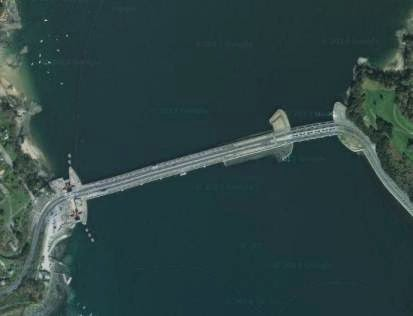
\includegraphics{/home/lewi/geaWaves/gea-waves/_hugo/content/tfg/1MEMORIA/imgMemoria/54-centralRance.jpg}
  \caption{}
  \end{figure}

  Figura 5.4: Imagen de la central Mareomotriz de
  \href{http://ireneu.blogspot.com.es/2014/07/la-ecologica-y-desastrosa-central.html}{La
  Rance}

  En 2011,
  \href{https://www.blogenergiasostenible.com/central-energia-mareomotriz-rance-mas-grande-mundo/}{la
  central de Rance pasó a ser la segunda planta más grande del mundo},
  tras inaugurarse la central mareomotriz de Sihwa Lake en Korea del
  Sur, con 10 turbinas de 25,4 MW y diámetro de 14 metros. Con una
  variación de nueve metros del nivel de las costas, la planta produce
  \href{http://world.kbs.co.kr/spanish/archive/program/news_issue.htm?no=22473}{554
  millones de kilovatios al año}. 
\item
  \textbf{La energía térmica oceánica o maremotérmica (OTE)}: La
  diferencia de temperaturas entre la superficie de los océanos
  calentados por el sol y las profundidades más frías, constituyen otra
  fuente de energía.

  Las zonas térmicamente favorables se encuentran en las regiones
  ecuatoriales y subtropicales. El Instituto de Energía del Océano de la
  Universidad de Saga en Japón es el mayor centro investigador de esta
  tecnología del mundo, en 1981 desarrolló e instaló una planta de 100kW
  en la isla de Nauru. Asimismo, Hawaii es uno de los emplazamientos
  idóneos para el aprovechaimento de esta energía, por las altas
  temperaturas superficiales y grandes profundidades alcanzables , es
  allí donde el gobierno americano tiene un laboratorio de investigación
  y una planta piloto de 10 MW, que pretenden ampliar a 100 MW para el
  año 2020.
  (\url{https://www.blogenergiasostenible.com/plantas-energia-maremotermica-mas-grandes-mundo/})
\item
  \textbf{La energía del gradiente salino}: Se basa en el
  aprovechamiento de la energía por la diferencia en la concentración de
  sal entre el agua dulce y el agua del mar, mediante una membrana
  osmótica.

  Respecto a esta técnica, en 2016,
  \href{https://www.carnegiece.com/wave/}{Carnegie, clean energy},
  instaló la tecnología CETO, primera mundialmente, convierte la energía
  cinética del oleaje y desaliniza el agua a través de la osmosis
  inversa.

  \href{https://www.carnegiece.com/project/ceto-6-garden-island/}{CETO
  6}, ubicado en la costa de Garden Island, al oeste de Australia, tiene
  una capacidad de 1 MW. Está respaldado por el gobierno federal a
  través de una subvención de la Agencia Australiana de Energía
  Renovable (ARENA) de 11 millones de dólares, así como de un préstamo
  del Commonwealth Bank of Australia.

  \begin{figure}
  \centering
  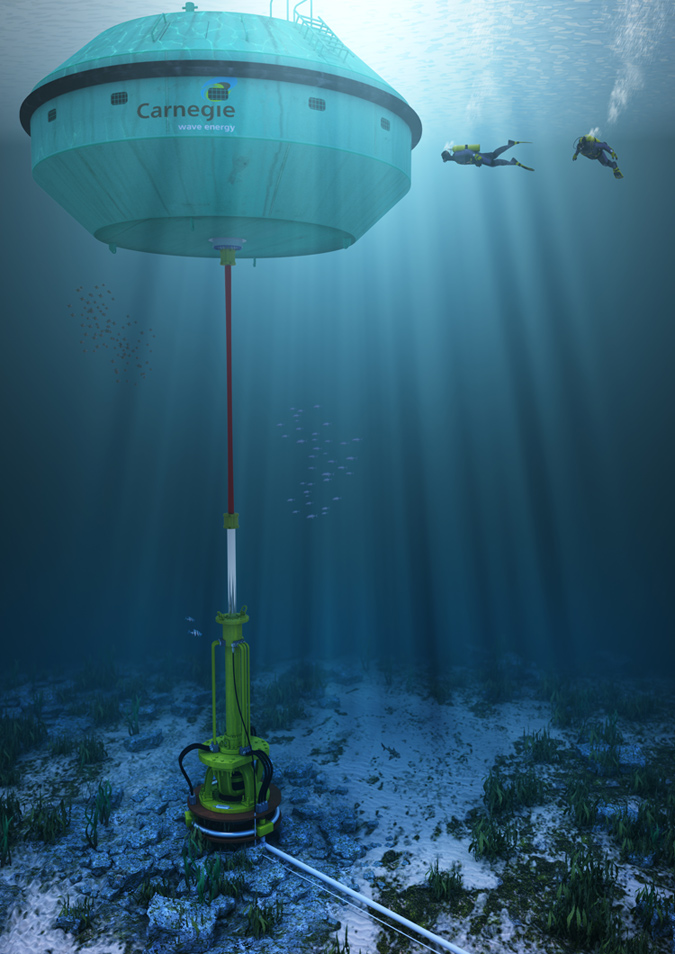
\includegraphics{/home/lewi/geaWaves/gea-waves/_hugo/content/tfg/1MEMORIA/imgMemoria/55-CETO.jpg}
  \caption{}
  \end{figure}

  Figura 5.5: By Carnegie Wave Energy Limited - Supplied by Carnegie
  Wave Energy Limited., CC BY-SA 3.0,
  {[}\url{https://commons.wikimedia.org/w/index.php?curid=31753495}{]}

  El concepto del diseño es la es la culminación del trabajo que comenzó
  en 2013 e incorpora lecciones aprendidas del Perth Wave Energy Project
  (CETO 5), pruebas de tanques de olas en Escocia, así como estudios
  internos de diseño y modelado. Carnegie cuenta con numerosos proyectos
  de colaboraciones I+D,
  \href{https://www.carnegiece.com/partner/research-partners/}{Research
  Partners}.
\item
  \textbf{La energía de las corrientes}: Mediante turbinas hidráulicas
  se aprovecha la energía que llevan las corrientes submarinas para
  crear energía eléctrica.
\item
  \textbf{La energía de las olas o undimotriz}: Las olas producidas, en
  gran medida, por el viento también resultan una fuente de energía. 
\end{itemize}

Cada una de estas corresponden a técnicas de estudio diferentes. Ya que
en las costas del mar cantábrico se dispone de un alto potencial en
energía de las olas, se optará por el análisis más en profundidad de
esta última.

\subsubsection{5.3.1 Según el principio de captación}\label{header-n85}

El aprovechamiento de la energía de las olas puede analizarse en base al
principio de funcionamiento y de captación de energía:

\begin{itemize}
\item
  Sistemas pasivos o estáticos: son aquellos en los que la estructura
  está inmóvil durante todo el proceso de conversión, de modo que la
  energía se genera sólo con el propio movimiento de las partículas de
  agua {[}Pinilla Martín, 2007{]}. 
\item
  Sistemas activos u oscilantes: aprovechan el movimiento relativo entre
  las partes fijas y las móviles del dispositivo. Existen dos tipos:

  \begin{itemize}
  \item
    El oleaje actúa directamente sobre el cuerpo móvil. La convesión
    primaria se basa en el movimiento relativo entre dos cuerpos.
  \item
    En la conversión secundaria, el oleaje actúa sobre una interfaz
    agua-aire, de modo que la ola desplaza al aire, que desplaza a su
    vez al cuerpo móvil. {[}Fernández Díez, 2002{]} 
  \end{itemize}
\end{itemize}

\begin{figure}
\centering
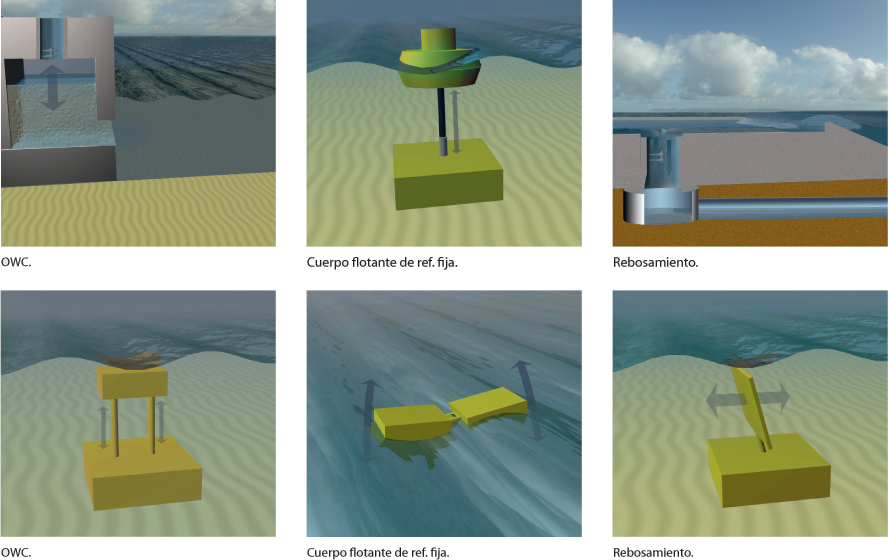
\includegraphics{/home/lewi/geaWaves/gea-waves/_hugo/content/tfg/1MEMORIA/imgMemoria/56-sistOlas.png}
\caption{}
\end{figure}

Figura 5.6: Sistemas de aprovechamiento del oleaje
{[}\url{www.aquaret.com}{]}

\subsubsection{5.3.2 Según la orientación respecto al
oleaje}\label{header-n106}

Los captadores pueden clasificarse de diferentes formas, una de ellas es
según la orientación respecto al oleaje y la forma:

\begin{itemize}
\item
  \textbf{Absorbedores puntuales}: Son estructuras de tamaño reducido en
  comparación a el oleaje incidente. Generalmente se colocan varios
  dispositivos agrupados siguiendo una línea. Concentran el oleaje en un
  punto. 
\item
  \textbf{Atenuadores}: Tienen forma alargada y se colocan paralelos a
  la dirección de avance de la ola. Captan la energía de manera
  progresiva. Las fuerzas a ambos lados de la estructura se compensan,
  de manera que requieren un sistema de amarre menos resistente que en
  el caso de los totalizadores. 
\item
  \textbf{Totalizadores o terminadores}: de forma alargada, se colocan
  perpendiculares a la dirección de avance de las olas. Requieren un
  sistema de amarre más resistente que los atenuadores. {[}Cavia del
  Olmo{]}
\end{itemize}

\begin{figure}
\centering
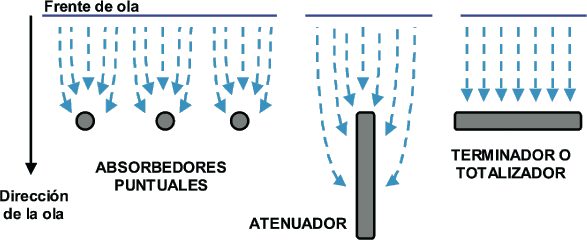
\includegraphics{/home/lewi/geaWaves/gea-waves/_hugo/content/tfg/1MEMORIA/imgMemoria/57-clasf-forma.png}
\caption{}
\end{figure}

Figura 5.7: Clasificación de dispositivos de energía de las olas por su
forma {[}P. Ibáñez, 2008{]}

\subsubsection{5.2.3 Según la localización}\label{header-n123}

En general, a medida que aumenta la distancia a la costa la densidad de
energía es mayor, pero la supervivencia está más comprometida y existe
una mayor complicación para el transporte de la energía generada, por lo
que hay que encontrar un compromiso entre la supervivencia del
dispositivo y la densidad de energía. Se reconocen tres zonas:

\begin{figure}
\centering
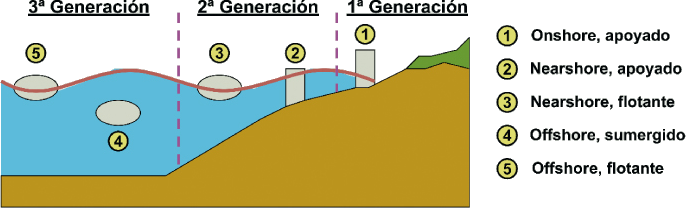
\includegraphics{/home/lewi/geaWaves/gea-waves/_hugo/content/tfg/1MEMORIA/imgMemoria/58-clasf-ubicacion.png}
\caption{}
\end{figure}

Figura 5.8: Clasificación de dispositivos según su ubicación
{[}\url{https://revista-anales.icai.es/web/n_14/seccion_8.html}{]}

\paragraph{5.2.3.1 En la costa (onshore)}\label{header-n130}

Presentan la ventaja de tener un coste de instalación y mantenimiento
menor, puesto que son de fácil accceso, además, el transporte de la
energía a la red presenta menos impedimentos. Sin embargo, disponen de
un potencial energético menor que el explotable mar adentro, aunque se
pueda ver compensado por efectos de concentración de energía por
refracción o difracción. Un solo convertidor puede ser suficiente para
cubrir determinadas necesidades a pequeña escala.

Los dispositivos que se pueden encontrar son:

\begin{itemize}
\item
  Columna de agua oscilante (Ozcillating Water Column, OWC)

  Constan de una estructura parcialmente sumergida hueca por la parte de
  abajo, dentro de la cual hay una cámara de aire por debajo del nivel
  del mar. El movimiento del oleaje se traduce en presión sobre el aire
  situado en el interior, que se expansiona y comprime accionando
  turbina que a su vez acciona el generador.

  Los rendimientos suelen ser del 30-50\% y pueden estar instalados en
  estructuras fijas, móviles o flotantes, o bien sobre el lecho rocoso
  de la costa o aprovechando instalaciones portuarias. La potencia a la
  que operan oscila entre los 100 y 500 KW.

  Esta técnica ha sido una de las más utilizadas:

  \begin{itemize}
  \item
    LIMPET (Land Installed Marine Powered Energy Transformer)

    El dispositivo fue desarrollado por la compañía británica
    \textbf{WaveGen Ltd.} en diciembre del 2000 en la Isla de Islay en
    la costa oeste de escocia, donde existe un flujo de energía
    disponible de entre 15 y 25 KW/m. Consta de dos turbinas tipo Wells
    cada una de las cuales tiene una capacidad instalada de 250 kW.
    Dicho dispositivo se encuentra conectado a la red, ha demostrado ser
    estructuralmente resistente a condiciones extremas de temporal con
    mantenimiento mínimo y en la actualidad sirve como base experimental
    para desarrollar nuevas tecnologías. Esta planta ha estado operando
    con éxito durante once años como un proyecto de demostración.

    En 2005, \textbf{Voith Hydro Power Generation}, filial de Voith
    ,compró Wavegen.

    \begin{figure}
    \centering
    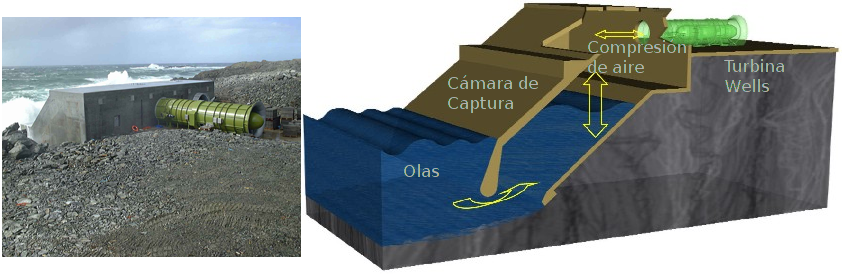
\includegraphics{/home/lewi/geaWaves/gea-waves/_hugo/content/tfg/1MEMORIA/imgMemoria/59-limpet.png}
    \caption{}
    \end{figure}

    Figuras 5.9: Fotografía y esquema de componentes de Limpet.
    {[}\url{www.wavegen.co.uk}{]}

    El diseño consta de tres compartimentos iguales y cuadrados
    inclinados 40º respecto a la horizontal que actúan como columna de
    agua. Se ha optimizado para reducir el impacto visual por su baja
    coronación y para ser de fácil instalación y mantenimiento.
  \item
    OWC Unión Fenosa (La Coruña)

    Es un sistema promovido por \textbf{Unión Fenosa} e instalado en
    Galicia, en la central térmica de Sabón. En 1990 se empezó la
    investigación del dispositivo que funciona no con una turbina
    accionada por aire como los anteriores, sino con medios mecánicos
    por flotación de un cuerpo sobre la columna de agua. Está situado en
    un pozo existente que se comunica con el mar, consta de un flotador
    de 6m de diámetro conectado a un dispositivo mecánico que transforma
    el movimiento ascendiente y descendiente de las olas en un giro que
    acciona el generador eléctrico. 
  \item
    Pico OWC (Portugal)

    Situada en la isla de Pico en las Azores, fue construida en 1998
    sobre un lecho rocoso a 8 metros de profundidad. Aunque en un
    principio no operaba correctamente debido a problemas técnicos y
    financieros, finalmente, de 2003 a 2006 se llevó a cabo un proyecto
    para recuperar el sistema. La potencia máxima de salida es de 400
    KW, se encuentra equipada con una turbina tipo Wells, con una cámara
    de 12x12 metros a cota del nivel medio del mar. Actualmente cubre
    parte de la demanda energética de la isla.

    \begin{figure}
    \centering
    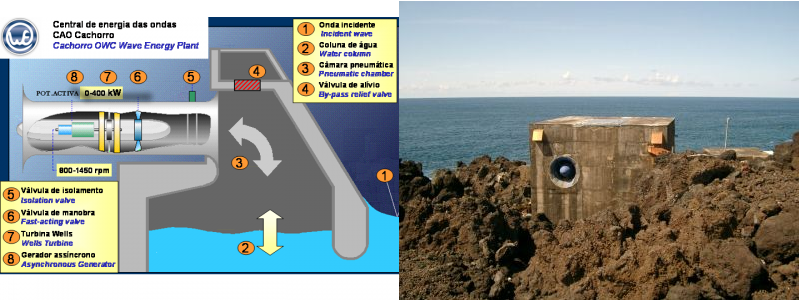
\includegraphics{/home/lewi/geaWaves/gea-waves/_hugo/content/tfg/1MEMORIA/imgMemoria/510-pico.png}
    \caption{}
    \end{figure}

    Figura 5.10: Esquema de componentes y fotografía de la planta OWC de
    Pico {[}\url{www.pico-owc.net}{]} 
  \item
    Mutriku, País Vasco

    Después de la exitosa demostración de LIMPET, en 2011 Voith Hydro
    Wavegen vendió la primera planta de energía comercial al Ente Vasco
    de Energía (EVE), conectada a la red española.
    \href{https://www.inverness-courier.co.uk/News/Inverness-firm-alunches-first-tidal-wave-project-16112011.htm}{Inverness-news
    16/11/2011}

    Ubicada en el dique del puerto, consta de 16 turbinas de 18,5 kW,
    con una potencia máxima de 480kW, genera unos 600 MWh/año.

    \begin{figure}
    \centering
    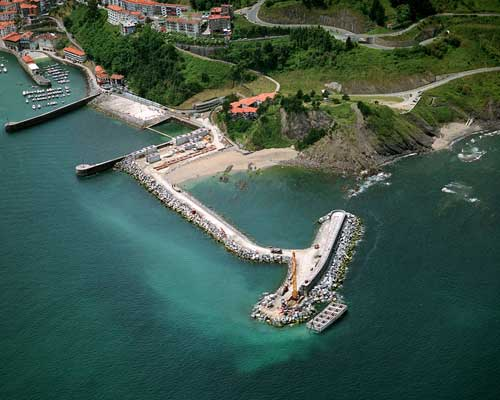
\includegraphics{/home/lewi/geaWaves/gea-waves/_hugo/content/tfg/1MEMORIA/imgMemoria/511-mutriku.jpeg}
    \caption{}
    \end{figure}

    Figura 5.11: Fase de construcción del sistema OWC
    {[}\url{http://www.interempresas.net/Energia/Articulos/101717-Energia-undimotriz-un-inmenso-potencial-aun-por-desarrollar.html}{]}

    La planta de energía utilizó tecnología desarrollada y suministrada
    por Voith Hydro Wavegen con un contrato por valor de 1,2 millones de
    euros (£ 1 millón). La inversión total del proyecto asciendió a 6,7
    millones, de los cuales 2,3 millones correspondieron a la
    instalación energética y fueron aportados por el Ejecutivo
    autonómico,
    \href{http://www.eitb.eus/es/noticias/sociedad/detalle/698089/mutriku-tiene-primera-planta-suministra-energia-olas/}{eitb-noticias
    08/07/2011.} El proyecto, también recibió asistencia financiera del
    Séptimo Programa Marco de la Comisión Europea,
    \href{https://www.power-technology.com/projects/mutriku-wave/}{Power-technology:
    Mutriku Wave Energy Plant}.

    En 2013 Voith Hydro decidió cerrar Wavegen por centrarse en
    proyectos de energía mareomotriz,
    \href{https://www.inverness-courier.co.uk/News/City-job-losses-as-giant-utility-firm-pulls-out-04032013.htm}{Inverness-news
    04/03/2013}.
  \item
    Sanze o boya Masuda (Japón)

    En 1983 se coloca un dispositivo en Sanze destinado a la
    investigación. La potencia máxima de generador era de 40 kW, formado
    por una boya con un sistema que actúa por el principio de la cavidad
    resonante en su interior, y acciona una turbina de aire comprimido.
    Funcionó durante muchos años hasta que se decidió examinar su
    respuesta a la corrosión y fatiga.
  \item
    Kvaerner (Noruega)

    En 1985 se instala en Toftestallen un dispositivo de captación de
    energía de potencia 500 kW, que fue destruido por una tormenta en
    1988. Se diseñó sobre un acantilado vertical de 30m, con base de
    hormigón y tubo metálico de 10 m de diámetro. La olas entraban por
    la parte inferior del cilindro desplazando la columna de aire y
    accionando la turbina Wells instalada en el extremo superior. Daba
    servicio a una comunidad próxima de 50 casas.
  \end{itemize}
\item
  TAPCHAN (TAPered-CHANnel)

  Consta de una estructura en canal que se hace cada vez más estrecho de
  forma gradual, desde el nivel medio del mar hasta un depósito más
  elevado. A medida que el oleaje se propaga por el canal, la altura de
  ola se amplifica hasta que sobrepasa la estructura y entra al depósito
  de reserva, el cual proporciona un flujo continuo de agua a una
  turbina tipo Kaplan. Finalmente, el agua se devuelve al mar mediante
  una turbina convencional hidroeléctrica que genera electricidad.

  \begin{itemize}
  \item
    Toftestallen (Noruega)

    Prototipo promovido por \textbf{Norwave A.S.} y finalizadao en 1985.
    Su potencia máxima es de 400 kW, consta de un canal de 170 m de
    longitud con un desnivel de 4m por encima del nivel medio del mar.
    Desemboca a un depósito de \emph{8500} \(m^3\) de capacidad, que a
    su vez alimenta una turbina Kaplan de \emph{0,35 MW}. La instalación
    estuvo funcionando durante tres años hasta que fuera destruida por
    una tormenta. Una segunda planta estuvo en funcionamiento hasta
    1991, con el mismo final. Hoy en día solo quedan las ruinas de lo
    que fueron, siendo un ejemplo de lo difícil que puede resultar
    lidiar con las fuerzas de la naturaleza. Noruega fué líder mundial
    en la investigación de la energía de las olas en la década de los
    80, pero la falta de apoyo financiero golpeó al sector.
    {[}\url{https://coastlight.net/detaljer/4283/Toftestallen/}{]}

    \begin{figure}
    \centering
    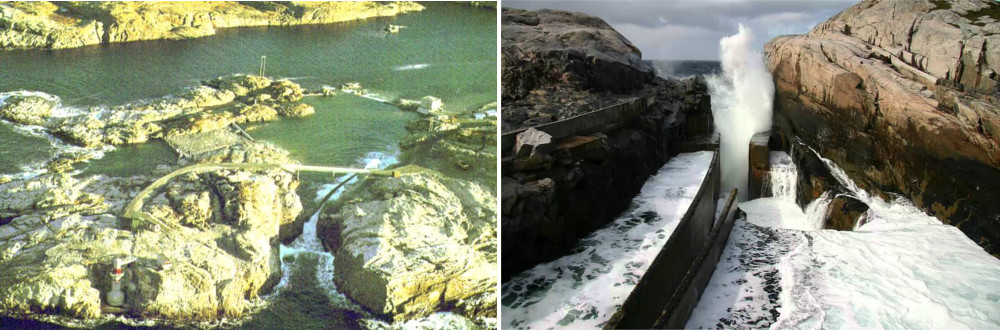
\includegraphics{/home/lewi/geaWaves/gea-waves/_hugo/content/tfg/1MEMORIA/imgMemoria/512-tapchan.jpg}
    \caption{}
    \end{figure}

    Figuras 5.12: Fotografías de la planta de Toftestallen.
    {[}\url{https://www.pinterest.co.uk/pin/196539971214291734/}{]} y
    {[}\url{https://coastlight.net/detaljer/4283/Toftestallen/}{]}
  \end{itemize}
\item
  Pendulor

  Es un dispositivo de captación que se puede situar tanto en la costa
  como cerca de ella, basado en un péndulo oscilante movido por el
  oleaje. Japón ha sido el país pionero en el desarrollo de este tipo de
  tecnología, llevando a cabo modelos a escala real. Consiste en una
  cámara de hormigón armado de forma rectangular con un lado abierto al
  mar. En éste lado se dispone de una compuerta de acero articulada en
  la parte superior que recibe el empuje del oleaje. El movimiento
  oscilatorio de dicha compuerta acciona una bomba hidráulica conectada
  a un generador.

  \begin{itemize}
  \item
    Mururoa (Japón)

    Sistema desarrollado por \textbf{JAMSTEC}, prototipo instalado en el
    puerto de Mururoa. Presenta una eficiencia total del 55\%. Consta de
    un cajón de 8 metros de altura con dos cámaras de (2,3x7,5)m, el
    péndulo tiene una altura de 7,5 metros y un ancho de 2 metros que
    entra en funcionamiento al alcanzar los 14º, oscilando como máximo a
    30º. Su potencia máxima es de 15 kW.

    \begin{figure}
    \centering
    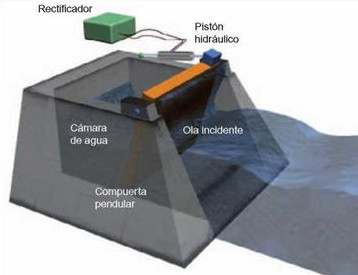
\includegraphics{/home/lewi/geaWaves/gea-waves/_hugo/content/tfg/1MEMORIA/imgMemoria/513-pendulor.jpg}
    \caption{}
    \end{figure}

    Figura 5.13: Esquema del dispositivo pendulor.
    {[}\url{http://energyprofessionalsymposium.com/?p=36743}{]} 
  \end{itemize}
\end{itemize}

\paragraph{5.2.3.2 Cerca de la costa (nearshore)}\label{header-n228}

Son aquellos dispositivos situados a una distancia máxima de 500 metros
de la costa y a una profundidad deentre 20 y 30 metros, pueden estar o
bien apoyados en el fondo o bien ser flotantes. Igualque en el caso de
los aparatos en la costa, presentan la ventaja detener un coste
deinstalación y mantenimiento menor que en aguas profundas. El mayor
inconveniente es, además del impacto visual, que su instalación implica
la modificación de la dinámica costera.

\begin{itemize}
\item
  OWC Port Kembla, Australia

  Proyecto desarrollado por \textbf{Energetech} en 2005, situado a 200
  metros de Port Kembla. Prototipo de columna de agua oscilante que
  utiliza una pared parabólica para focalizar la energía de las olas,
  alcanzando alturas de 2,5 a 3 veces superiores. Con olas de 2 m y
  periodos de 7 segundos, genera 320 kW, de los cuales una parte se
  emplea para desalinizar agua a bordo del dispositivo. Tiene unas
  dimensiones de 36x35 metros y 18 metros de profundidad, genera una
  potencia máxima de 500kW. Además, desarrollaron una turbina de palas
  orientables (Denniss-Auld) para transformar el flujo ascendente y
  desdendente en giro unidireccional. Debido a las condiciones
  climáticas extremas imprevistas en 2010, el prototipo MK3 se liberó de
  sus amarres. La unidad se recuperó con éxito para ser conectada
  nuevamente a la red. Posteriormente, en ese mismo año, la unidad fue
  eliminada de manera
  segura.{[}\url{https://en.wikipedia.org/wiki/Oceanlinx}{]}

  \begin{figure}
  \centering
  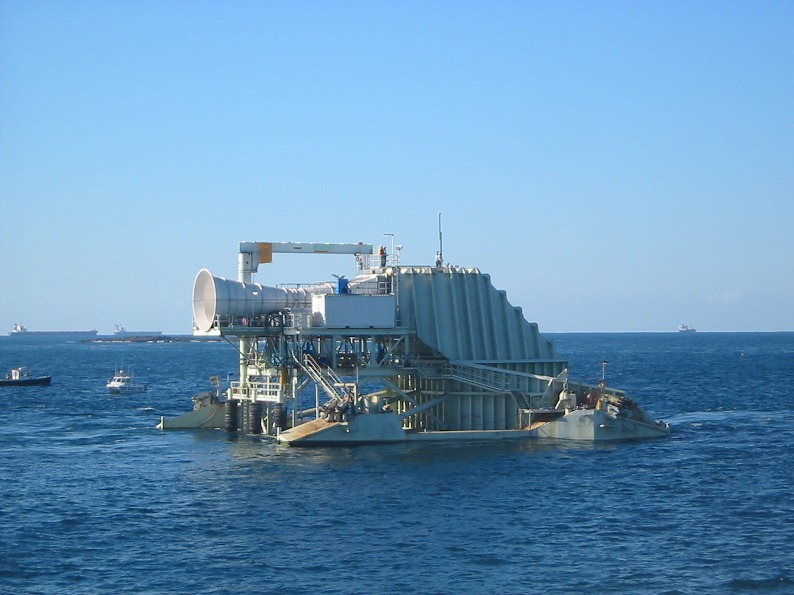
\includegraphics{/home/lewi/geaWaves/gea-waves/_hugo/content/tfg/1MEMORIA/imgMemoria/514-Australia-oceanlix.jpg}
  \caption{}
  \end{figure}

  Figura 5.14: Proyecto de Oceanlix greenWAVE en Port MacDonnell.
  {[}\url{https://www.offshorewind.biz/2013/09/04/australia-construction-starts-on-oceanlinxs-wave-energy-project/}{]}

  En 2007, la compañía cambió su nombre por Oceanlinx y la tecnología
  siguió en desarrollo. En 2014, la estructura greenWAVE quedó varada en
  la bahia de Yankalilla después de que surgieran dificultades mientras
  la remolcaban desde Port Adelaide hasta Port MacDonnell,
  \href{https://www.offshorewind.biz/2015/04/14/greenwave-still-stranded-off-south-australia/}{Business
  Guide}. Esto llevó a la compañía Oceanlinx a ingresar en la
  administración judicial antes de que su tecnología, propiedad
  intelectual y marca comercial fueran vendidas a \textbf{Wave Power
  Renewables Limited} en Hong Kong. Desde entonces estos han seguido
  desarrollando la tecnología, habiendo logrado 15 patentes y 18 en
  proceso. La versión más avanzada a gran escala se lanzará en el primer
  trimestre de 2018.\\
\item
  Oyster WEC (Wave Energy Converter), Reino Unido.

  Aquamarine Power, fundada en 2005 en Edinburgo, implementó y probó dos
  dispositivos Oyster a gran escala en EMEC (European Marine Energy
  Centre): el Oyter 1 de 315kW y el Oyster 800 de 800kW. Trabaja con un
  módulo anclado al fondo marino que con el movimiento oscilatorio mueve
  unos pistones, que a su vez entregan el agua a presión a una unidad de
  transformación hidroeléctrica ubicada en la costa. Trabaja a
  profundidades de 10 a 12 metros, dando una potencia máxima de entre
  300 y 600 kW.\\

  Oyster 800 se conectó a la red en 2012 en la zona de pruebas de Billia
  Croo (EMEC), hasta el cierre del programa que finalizó en 2015, cuando
  la empresa dejó de operar.
  (\url{http://www.emec.org.uk/about-us/wave-clients/aquamarine-power/})

  \begin{figure}
  \centering
  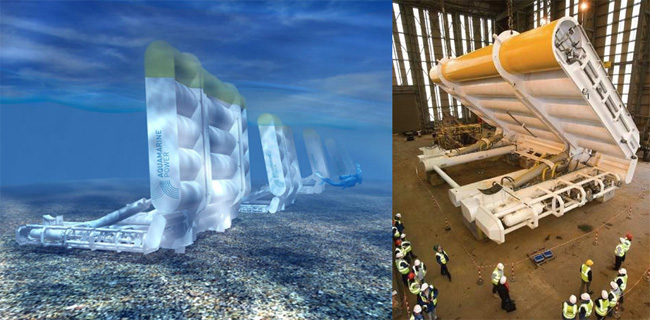
\includegraphics{/home/lewi/geaWaves/gea-waves/_hugo/content/tfg/1MEMORIA/imgMemoria/515-oyster.jpg}
  \caption{}
  \end{figure}

  Figuras 5.15: Esquema y fotografía del sistema Oyster
  {[}\url{www.aquamarinepower.com}{]}
\item
  Wave Roller

  Sistema desarrollado por AW Energy Oy a escala de laboratorio entre
  los años 1999 y 2004. En 2005 se construyó un prototipo a escala (1:3)
  que probó la viabilidad del dispositivo. En la actualidad existe un
  prototipo a escala real instalado en Peniche (Portugal).

  Consiste en una placa anclada al fondo del mar por la parte inferior,
  la cual se mueve por el movimiento oscilatorio de las olas en el
  fondo. Se coloca a una profundidad de aproximadamente 7 a 15 metros,
  proporcionando una potencia nominal de 13 kW por placa (se disponen de
  3 a 45 placas). Puesto que se encuentra sumergido, no presenta
  problemas de impacto visual y acústico.
\end{itemize}

\begin{figure}
\centering
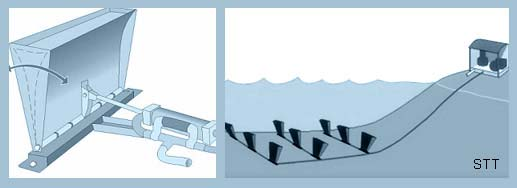
\includegraphics{/home/lewi/geaWaves/gea-waves/_hugo/content/tfg/1MEMORIA/imgMemoria/516-waveroller.jpg}
\caption{}
\end{figure}

Figura 5.16: Esquema del funcionamiento de
WaveRoller.{[}\href{http://www.see.murdoch.edu.au/resources/info/Tech/wave/}{School
of Engineering and Energy, Murdoch University}{]}

\href{http://www.aw-energy.com/}{www.aw-energy.com}{]}

\begin{itemize}
\item
  Mighty Whale

  El dispositivo fue desarrollado en Japón en 1998, y se puso en
  funcionamiento en mayo del 2002 en la bahía de Gocazo. Es una
  estructura de 50 x 30 metros capaz de generar con un frente de 30m y
  40m de longitud una potencia de 110kW, con una eficacia del 60\%
  aproximadamente. El principio por el cual genera la electricidad es
  debido a las presiones y succiones de aire que provoca la agitación
  del oleaje.

  \begin{figure}
  \centering
  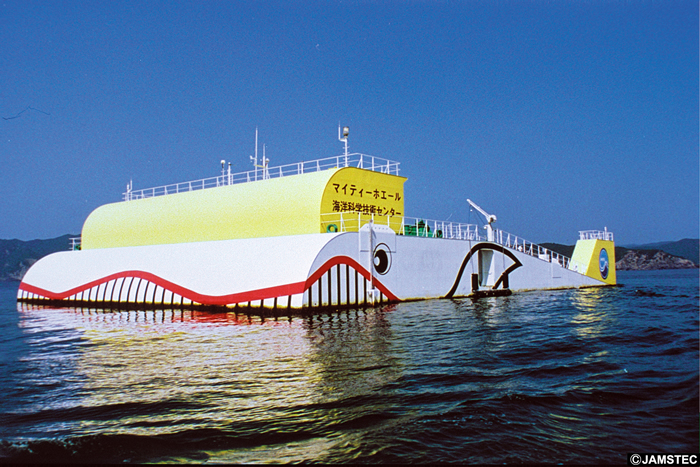
\includegraphics{/home/lewi/geaWaves/gea-waves/_hugo/content/tfg/1MEMORIA/imgMemoria/517-MightWhale.jpg}
  \caption{}
  \end{figure}

  Figura 5.17: Imagen del Mighty
  Wave.{[}\href{http://www.jamstec.go.jp/}{www.jamstec.go.jp}{]}
\end{itemize}

\paragraph{5.2.3.3 Mar a dentro (offshore)}\label{header-n279}

La principal ventaja que representan respecto a los anteriores
dispositivos es que en aguas profundas (\textgreater{}40m) existe un
potencial energético mayor, ya que el oleaje todavía no ha experimentado
pérdidas. Sin embargo, al ser a profundidades mucho mayores, aparecen
otras dificultades añadidas como: el coste y la complejidad de
instalación, difícil accesibilidad para mantenimiento y reparación, la
esctructura y los sistemas de amarre deben resistir grandes esfuerzos e
interferencias con el tráfico marítimo.

Los prototipos estudiados para esta ubicación son, entre otros:

\begin{itemize}
\item
  Archimedes wave swing (AWS)

  Se trata de un sistema de conversión que se encuentra totalmente
  sumergido entre los 40 y 100m de profundidad. Está formado por dos
  cilindros: el primero se encuentra fijado al fondo y el otro hace la
  función de flotador, desplazándose verticalmente debido a la
  incidencia del oleaje.

  \begin{figure}
  \centering
  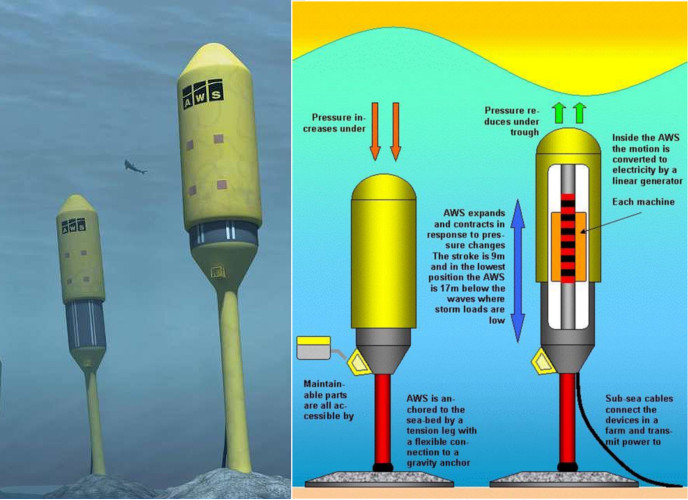
\includegraphics{/home/lewi/geaWaves/gea-waves/_hugo/content/tfg/1MEMORIA/imgMemoria/518-aws.jpg}
  \caption{}
  \end{figure}

  Figuras 5.18: Esquema de funcionamiento. \href{www.awsocean.com}{Luc
  Hamilton, 2006} y
  {[}\url{https://www.researchgate.net/figure/Archimedes-Wave-Swing-by-AWS-Ocean-Energy_fig9_283368443}{]}

  \begin{itemize}
  \item
    Viana do Castello (Portugal)

    Fué la primera planta piloto instalada, en 2004. En este prototipo
    el sistema de sujeción era mediante un pontón con 4 torres que se
    llenaban de agua al sumergirse. La carrera nominal era 7 m (subida y
    bajada del flotador), y la velocidad nominal 2,2 m/s. El prototipo
    se probó durante 7 meses a una profundidad de 43 m y con una
    potencia máxima de 2 MW, conectado a la red.

    \begin{figure}
    \centering
    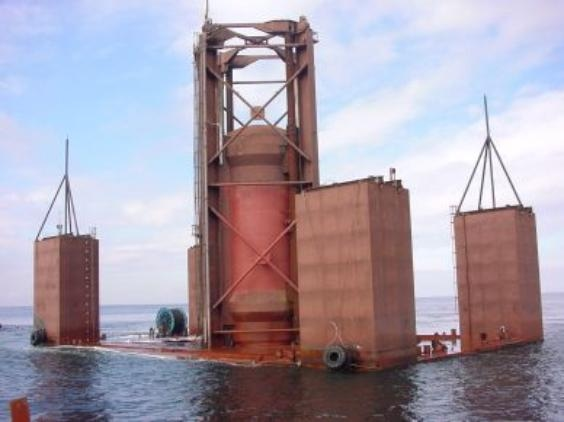
\includegraphics{/home/lewi/geaWaves/gea-waves/_hugo/content/tfg/1MEMORIA/imgMemoria/519-AWSportugal.jpg}
    \caption{}
    \end{figure}

    Figura 5.19: Sistema AWS en Viana do Castello
    (Portugal){[}\url{www.awsocean.com}{]} 
  \item
    Lyness, Orkney

    En 2014, \textbf{AWS Ocean Energy Ltd} finalizó la instalación a
    gran escala del generador de energía AWS-III en el muelle de Lyness.
    Con el objetivo de demostrar su funcionamiento, durabilidad, impacto
    ambiental, ruido y vibraciones. Los resultados de las pruebas fueron
    muy positivos y están trabajando en la siguiente etapa de desarrollo
    dentro de una viabilidad comercial.
    {[}\url{http://www.awsocean.com/projects.html}{]}
  \end{itemize}
\item
  Powerbuoy

  Tecnología desarrollada por \textbf{OPT} (Ocean Power Technologies) de
  Estados Unidos. El sistema consiste en aprovechar el movimiento
  vertical y pendular del oleaje a través de una boya de unos 2 a 5
  metros de diámetro abierta por la parte inferior. Las boyas obtienen
  la energía mediante un sistema hidráulico que aprovecha el movimiento
  relativo entre el flotador y el mástil de la boya. El sistema bombea
  un fluido (aceite) a alta presión que a su vez acciona un generador
  eléctrico. El rango de potencias de salida depende de la ubicación, de
  3 Kw hasta 15 kW.

  \begin{figure}
  \centering
  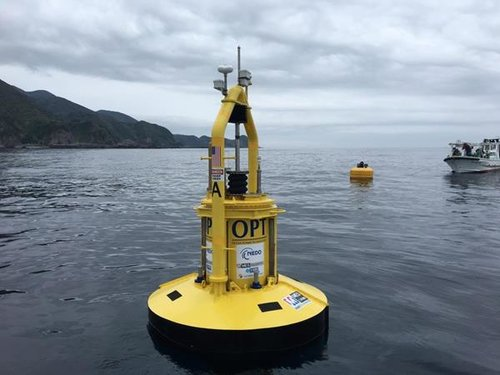
\includegraphics{/home/lewi/geaWaves/gea-waves/_hugo/content/tfg/1MEMORIA/imgMemoria/520-powerbuoy.jpg}
  \caption{}
  \end{figure}

  Figura 5.20: Dispositivo PowerBuoy de Atlantic City
  {[}\url{www.oceanpowertechnologies.com}{]}

  Se han llevado a cabo tres proyectos situados en el Atlántico y en el
  Pacífico:

  \begin{itemize}
  \item
    Oahu (Hawai)

    Desarrollado entre 2004 y 2007 con el objetivo de utilizar la
    energía del oleaje para las bases de la marina norteamericana. El
    parque de olas estaba situado a una profundidad de 30 metros con una
    potencia de hasta 1MW. 
  \item
    Atlantic City (New Jersey)

    Parque operativo desde octubre del 2005 para demostrar la viabilidad
    del sistema de captación energética en el estado de Nueva Jersey. La
    boya es de 5 metros de diámetro y 14 metros de longitud. Se
    encuentra situada a una profundidad de 18 metros con una potencia
    nominal de 40kW.
  \item
    Santoña (España)

    El proyecto se empezó a desarrollar en 2006 para \textbf{Iberdrola
    S.A.}, con el objetivo de evaluar la viabilidad del sistema en la
    costa norte de España. En 2008, fué la primera planta de este tipo
    operativa en Europa. Participada por Iberdrola (60\%), TOTAL (10\%),
    OPT (10\%), el Instituto para la Diversificación y el Ahorro
    Energético, IDAE (10\%) y la Sociedad para el Desarrollo de
    Cantabria, SODERCAN (10\%). En la primera fase, que incluye la
    infraestructura eléctrica marina costó unos 3 millones de euros. Se
    dispuso una boya de 40 kW sin conexión a la red eléctrica,
    suministrada por OPT, formada por un flotador de unos siete metros
    de diámetro, un fuste (compartimento cilíndrico estanco) donde se
    aloja el sistema de transformación de la energía de unos 20 metros
    de largo y un estabilizador de aproximadamente 10 metros. Constando
    de un sistema de amarre de tres boyas ancladas al lecho marino a 50
    metros de profundidad, situada a 4 kilómetros de la costa e
    inicialmente se puso una potencia nominal de 1,35 MW.

    El sistema de transformación de la energía, denominado Power Take
    Off (PTO), está compuesto por una serie de módulos internos, a
    través de los cuales se capta y transforma la energía de las olas
    para almacenarla y, posteriormente, evacuarla en condiciones
    óptimas.

    \href{https://www.scribd.com/document/328163965/La-Fuerza-de-Las-Olas}{"La
    energía undimotriz se abre paso entre las renovables" La fuerza de
    las olas 2008}\\
  \end{itemize}
\item
  Aquabuoy

  Sistema desarrollado por Aquaenergy Group. Consta de una boya flotante
  que transforma el movimiento de subida y bajada provocado por el
  oleaje para transmitirlo a un pistón. Éste está unido a dos mangueras
  flexibles que funcionan como bombas de agua, impulsando el agua a
  presión a través de un tubo hacia el acumulador que se encuentra en la
  parte superior del dispositivo. El interior de la boya aloja un
  sistema turbina-generador que produce la electricidad. Renovables
  Finavera, actualmente, tiene proyectos de energía undimotriz en
  Portugal, Canadá, Estados Unidos y Sudáfrica.

  \begin{figure}
  \centering
  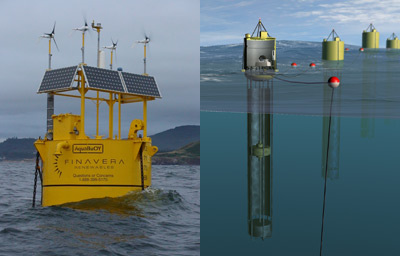
\includegraphics{/home/lewi/geaWaves/gea-waves/_hugo/content/tfg/1MEMORIA/imgMemoria/521-AquaBuOY.jpg}
  \caption{}
  \end{figure}

  Figura 5.21: Dipositivo Aquabuoy de Finavera Renewables
  \url{http://www.global-greenhouse-warming.com/Finavera-aquabuoy.html}{]}

  \begin{itemize}
  \item
    Bahia de Maca (EEUU)

    Fue impulsado debido a que presentaba condicionantes favorables:
    profundidad cerca de la costa, buen clima de oleaje y demanda
    energética en la zona. Una boya piloto se instaló en 2003 a una
    profundidad de más de 50 metros y diámetro y longitud de 6 y 30
    metros respectivamente. La potencia máxima de dicho dispositivo fué
    de 250kW.
  \end{itemize}
\end{itemize}

\begin{itemize}
\item
  Pelamis wave power

  Sistema desarrollado por la empresa británica \textbf{Pelamis Wave
  Power Ltd}, anteriormente conocida como Ocean Power Delivery Ltd. La
  idea partía de uno de los primeros dispositivos en estudiarse, el
  Salter Duck {[}Salter, 1974{]}. A lo largo de los años la idea ha ido
  evolucionando para dar paso a nuevos sistemas como la tecnología
  Pelamis.

  El dispositivo Pelamis está formado por una estructura cilíndrica
  semisumergida cuyo eje está orientado paralelamente a la dirección de
  propagación del oleaje. Se encuentra articulada en varios puntos que
  conforman nodos móviles con dos grados de libertad: vertical y
  horizontal. El movimiento relativo entre las partes articuladas
  acciona un sistema hidráulico de 4 pistones que alimenta un depósito a
  presión que, a su vez, actúa sobre un generador eléctrico. Se
  encuentra anclado al fondo por un sistema de pesos y flotadores que
  impide que vaya a la deriva sin restringir la oscilación del
  artefacto.

  \begin{figure}
  \centering
  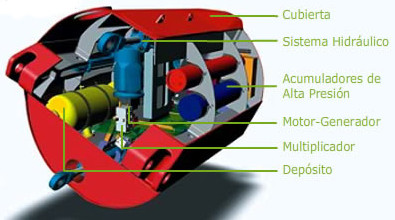
\includegraphics{/home/lewi/geaWaves/gea-waves/_hugo/content/tfg/1MEMORIA/imgMemoria/522-pelamis-scheme.jpg}
  \caption{}
  \end{figure}

  Figura 5.22: Esquemas de funcionamiento del dispositivo Pelamis
  {[}\url{http://www.eve.eus/La-energia/Infografias/La-energia-del-mar/La-energia-del-mar.aspx?lang=es-ES}{]}

  \begin{itemize}
  \item
    Aguaçadoura (Portugal)

    El proyecto empezó en 2005 y consiste en tres dispositivos Pelamis
    situados a 5 km de la costa norte de Portugal con capacidad de 2,25
    MW en total (cada uno de 750 kW). Es el primer parque de olas con
    pretensiones comerciales, se planificaron otros 28 convertidores,
    como parte de la segunda fase, para generar 22,5 MW para la empresa
    energética estatal Energías de Portugal. Sin embargo, los primeros
    tres generadores tuvieron que ser remolcados al puerto, tras cuatro
    meses de su puesta en servicio debido a problemas técnicos. La
    crisis financiera mundial del 2008 hizo que la reinstalación fuera
    aún más difícil y desde entonces ha permanecido cerrada.

    \url{https://www.power-technology.com/projects/pelamis/}
  \item
    Orkney (Escocia)

    Pelamis Wave Power (PWP), fundada en 1998, con sede en Edimburgo, en
    2004 demostró su primer prototipo a escala real. Se construyó con
    cuatro dispositivos Pelamis situados a 2 km de la costa oeste de
    escocia en el parque de pruebas del Centro Europeo de Energías
    Marinas (European Marine Energy Centre, EMEC), con una capacidad de
    3 MW. Entre 2004 y 2007 se llevó a cabo el dispositivo de segunda
    generación, el cual comprende 5 convertidores. En 2010 se llevó a
    Orkney y se instaló con éxito en el sitio de prueba de olas Billia
    Croo de EMEC. En 2014 PWP ingresó en administración y Wave Energy
    Scotland se hizo con sus activos, el dispositivo fué desmantelado.

    \begin{figure}
    \centering
    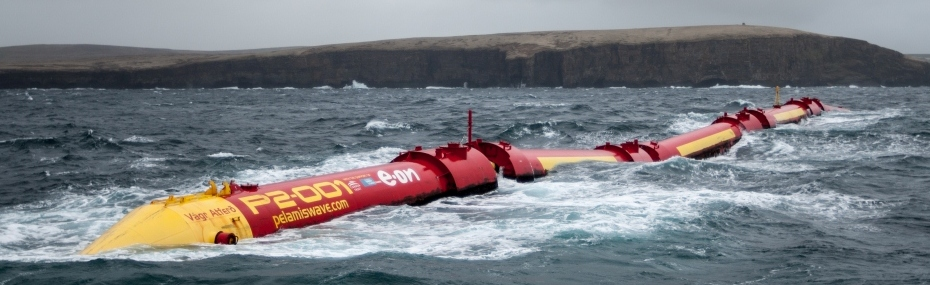
\includegraphics{/home/lewi/geaWaves/gea-waves/_hugo/content/tfg/1MEMORIA/imgMemoria/523-pelamisP002.jpg}
    \caption{}
    \end{figure}

    Figura 5.23: Imagen del convertidor pelamis P2-001
    {[}\url{http://www.emec.org.uk/about-us/wave-clients/pelamis-wave-power/}{]}

    EMEC adquirió el convertidor pelamis de ScottishPower Renewables,
    que estuvo desarrollando la tecnología antes de que PWP ingresara en
    administración. Actualmente con sede en Lyness, EMEC está explorando
    opciones para utilizar el dispositivo pelamis como plataforma de
    prueba, previendo que podría usarse para probar materiales,
    componentes u otras pruebas en mar
    abierto.(\url{http://www.emec.org.uk/press-release-emec-seeks-feedback-from-industry-for-p2-002/})
  \end{itemize}
\item
  Wave Dragon

  Sistema desarrollado por la compañía danesa Wave Dragon ApS. Empezó a
  estudiarse en 1998 a partir de modelos numéricos y ensayos en
  laboratorio.

  El corazón de la unidad es un gran depósito flotante, dos alas
  reflectoras concentran la potencia de las olas hacia una rampa, la
  cual conduce el agua al depósito. El agua vuelve al mar a través de
  una turbinas Kaplan de baja presión.

  Entre otros beneficios, cabe destacar que es el único convertidor bajo
  desarrollo que puede ser libremente escalado.

  \begin{itemize}
  \item
    Nissum Brending (Dinamarca)

    En 2003 un
    \href{\%5Bhttp://www.wavedragon.net/sea-testing-and-optimisation-of-power-production-on-a-scale-14-5-test-rig-of-the-offshore-wave-energy-converter-wave-dragon/}{proyecto
    Europeo}, con Wave Dragon ApS. (Denmark) y 5 entidades más de
    diferentes paises europeos, lanzó un prototipo a escala 1:4.5 en
    Nissum Bredning (the Danish Wave Energy Test Center), al norte de
    Dinamarca.

    En 2006 se instaló un prototipo modificado en otro sitio de pruebas
    con olas más energéticas. En mayo del 2008, se realizaron tareas de
    mantenimiento y reparación, y en 2009 el prototipo volvió a su lugar
    de origen para las pruebas finales. El prototipo fué diseñado a
    escala real para el oleaje de la zona cuya potencia media es de
    24kW/m, valor que corresponde a una escala de 1:5.2 para un clima de
    36 kW/m. La capacidad correspondiente a cada clima sería de 4 y 7 MW
    respectivamente.

    \begin{figure}
    \centering
    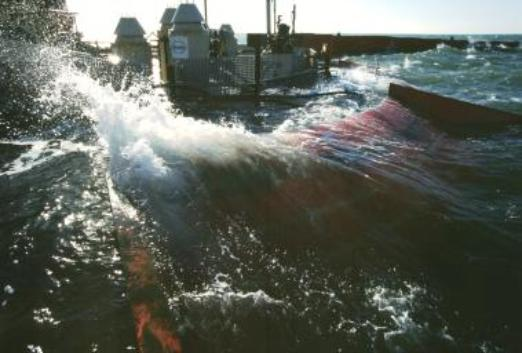
\includegraphics{/home/lewi/geaWaves/gea-waves/_hugo/content/tfg/1MEMORIA/imgMemoria/524-waveDragonNissum.jpg}
    \caption{}
    \end{figure}

    Figura 5.24: Wave Dragon en Nissum-Bedding (Earth Vision)
    {[}\url{http://www.wavedragon.net/prototype-testing-in-denmark/}{]}

    \begin{figure}
    \centering
    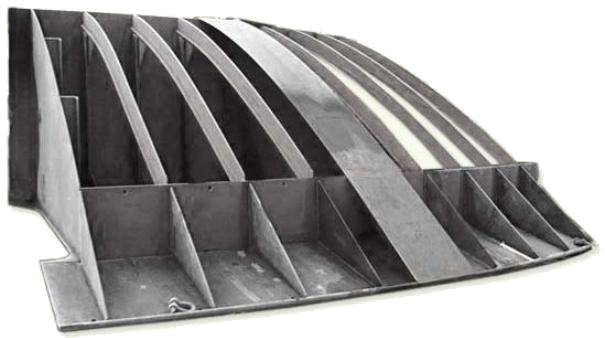
\includegraphics{/home/lewi/geaWaves/gea-waves/_hugo/content/tfg/1MEMORIA/imgMemoria/525-waveDragonRamp.png}
    \caption{}
    \end{figure}

    Figura 5.25: Diseño de rampa que optimiza la captura de agua
    {[}\url{www.wavedragon.net}{]} 
  \item
    TecDragon (Portugal)

    Proyecto desarrollado por TecDragon (Tecnologia da Energia das Ondas
    SA), compañía del Grupo Wave Dragon, ApS., en cooperación con
    investigadores portugueses y alemanes, cuyo objetivo es la
    instalación de un parque de olas de 50 MW.

    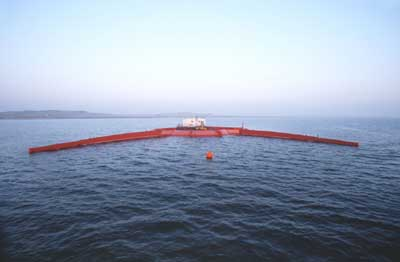
\includegraphics{/home/lewi/geaWaves/gea-waves/_hugo/content/tfg/1MEMORIA/imgMemoria/526-WaveDragonApS.jpg}

    Figura 5.26: \url{http://www.tecdragon.pt}
  \item
    Milford Haven

    Wave Dragon Wales Ltd. planeó instalar la demostración pre-comercial
    a gran escala del Wave Dragon ApS. en Gales en 2011/2012, con una
    capacidad de 7 MW, ubicada a dos o tres millas de St Ann's Head. Con
    el fin de obtener, durante tres a cinco años, experiencia
    operacional y análisis de las deficiencias en el tansporte de
    energía.

    Sin embargo, la crisis financiera causó retrasos en los planes de
    despliegue del primer dispositivo a gran escala y Wave Dragon Ltd.
    actualmente está buscando capital de riesgo.
    {[}\url{http://www.wavedragon.net/timetable/}{]}

    En 2015, Wave Dragon cerró la aplicación de la Sección 35 y dejó de
    trabajar en este sitio. Como sitio de pruebas, esta ubicación nunca
    habría sido comercialmente viable y desde 2013 comenzó a trabajar a
    gran escala comercial en 'Milla Fjord'.
    {[}\url{https://tethys.pnnl.gov/annex-iv-sites/wave-dragon-pre-commercial-demonstration-project}{]}
  \end{itemize}
\end{itemize}

\subsection{Actualidad del desarrollo tecnológico en España}\label{header-n430}

La gran disponibilidad de energía de oleaje de algunos países ha llevado
a gobiernos y empresas a financiar e impulsar programas de investigación
y desarrollo. Anteriormente, se ha visto como países europeos como
Dinamarca, Irlanda, Noruega, Reino Unido y Portugal apuestan fuertemente
en sus investigaciones en energía undimotriz. También a nivel mundial se
han llevado a cabo programas en sitios donde existe un gran potencial
como Australia, Canadá, Japón y Estados Unidos entre otros.

A nivel nacional, se han mencionado algunos proyectos, a continuación se
detalla su estado actual:

\begin{itemize}
\item
  Bimep

  Centro de ensayos en mar abierto, localizado en Armintza-Lemoiz
  (Bizkaia), cuenta con una superficie total de \(5,3 km^2\). En 2009 se
  instaló una boya oceanográfica en la zona, para medir parámetros como
  la altura y dirección del oleaje, velocidad y dirección de las
  corrientes y del viento, temperatura, etc. y transmitir los datos por
  satelite.

  \begin{figure}
  \centering
  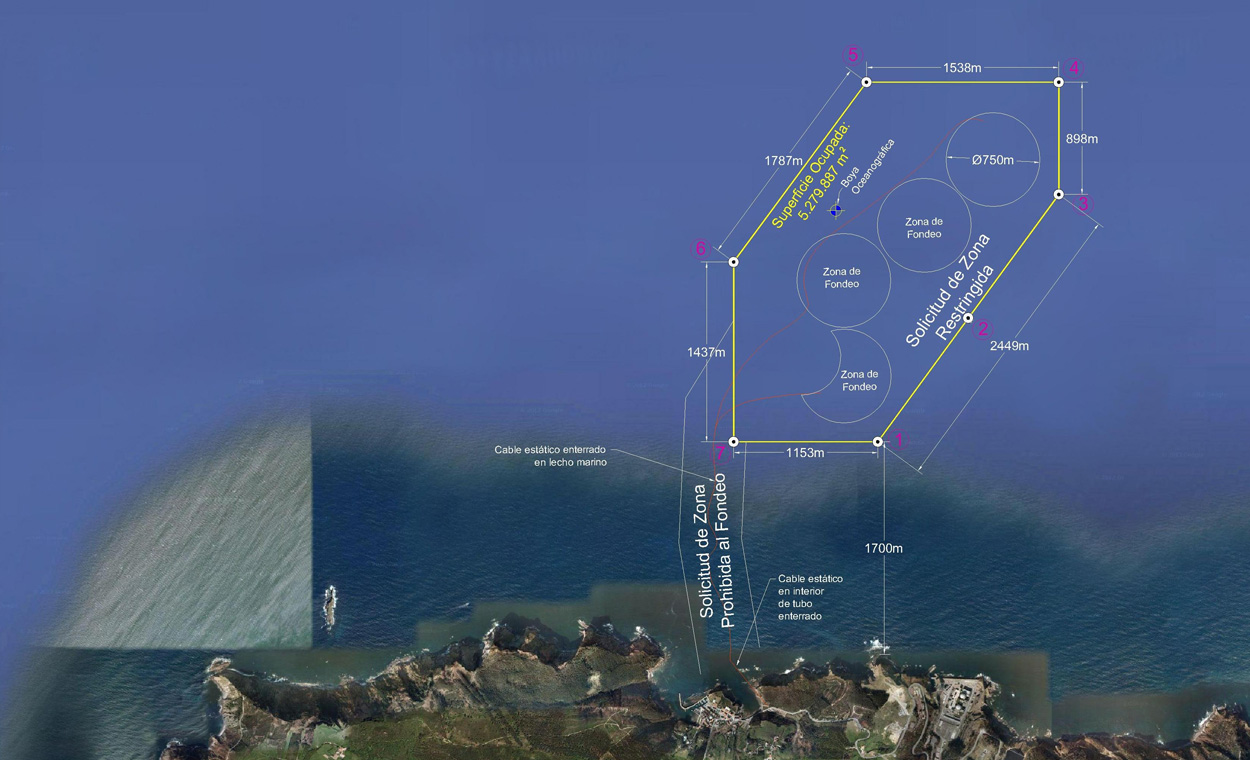
\includegraphics{/home/lewi/geaWaves/gea-waves/_hugo/content/tfg/1MEMORIA/imgMemoria/527-Ortofoto-bimep.jpg}
  \caption{}
  \end{figure}

  Figura 5.27: Fotografía de la disposición general,
  \href{http://bimep.com/sobre-bimep/localizacion-de-bimep/}{Localización
  de bimep}

  Se han realizado varios estudios detallados, medoambiental, de energía
  de las olas del País Vasco y de rutado del cable submarino, tal y como
  se detalla en el
  \href{http://bimep.com/sobre-bimep/desarrollo-del-proyecto/}{Desarrollo
  del Proyecto}. Además, se listan las empresas adjudicadas desde
  concursos públicos, para llevar a cabo cada tarea o suministrar
  equipamientos.

  \textbf{bimep} cuenta con
  \href{http://bimep.com/sobre-bimep/instalaciones/}{instalaciones}
  abiertas que permiten que los fabricantes de sistemas de generación
  renovable marina instalen sus equipos en ella, bien para
  explotación-demostración (generación de energía eléctrica) o bien para
  pruebas. Las características básicas de la infraestructura son:

  \begin{itemize}
  \item
    20 MW de potencia total.
  \item
    4 puntos de conexión para WECs.
  \item
    Facilidad de instalación, ensayo, pruebas y explotación.
  \item
    Centro de investigación asociado.
  \end{itemize}
\item
  Iberdrola Energías Marinas de Cantabria, S.A.

  El proyecto de investigación del convertidor Powerbuoy que mantenían
  en Santoña desde el 2008 y que estudiaban cómo desarrollar un enramado
  de 10 boyas que generasen potencia suficiente como para abastecer a
  2.500 viviendas quedó sin concluir.
  \href{http://www.eldiariomontanes.es/20131116/local/castro-oriental/abandono-proyecto-iberdrola-santona-201311161639.html}{Ref.:
  El Diario Montañés} -\textgreater{}
  \href{https://web.archive.org/web/20170904012830/http://www.eldiariomontanes.es/20131116/local/castro-oriental/abandono-proyecto-iberdrola-santona-201311161639.html}{Way
  Back Machine}

  En un momento tenso en las relaciones entre Iberdrola y el Gobierno
  por los recortes aplicados por el Ministerio de Industria al sector
  para intentar atajar el déficit tarifario, la empresa decidió bajarse
  de la iniciativa. La multinacional continuó su apuesta por la
  tecnología marina en Escocia, en las Islas de Orkney a través de la
  sociedad Scottish Power Renewables. En 2011 participó en la
  instalación del prototipo Pelamis P-2 en el EMEC en Orkney y, también,
  desarrollaron el proyecto Sound of Islay, de 10 MW de capacidad.

  La renuncia abocó a la desaparición de la empresa, Iberdrola Energías
  Marinas de Cantabria, S.A. en 2013, aunque, según fuentes de la
  eléctrica, la liquidación de esa sociedad no supone el fin del
  proyecto, que, aseguran, continúa, porque otros accionistas lo han
  "heredado".
  \href{https://www.vozpopuli.com/economia-y-finanzas/empresas/Iberdrola-Energia_marina-Cantabria_0_642535793.html}{Ref.:
  Voz Populi}
\item
  Mutriku wave plant, propiedad del EVE.

  En 2016 la central completó
  \href{https://tidalenergytoday.com/2016/07/19/mutriku-wave-plant-generates-over-1gwh-of-clean-power/}{5
  años de funcionamiento}, durante los cuales ha suministrado 1,3 GWh de
  potencia a la red eléctrica. A parte de producir energía de las olas,
  la planta también actúa como centro de pruebas para nuevas tecnologías
  de turbinas y sistemas de control.

  En mayo del 2017, se envió a la planta una turbina de aire bi-radial
  de Kymaner, después de haber sido ensayada en el laboratorio de la
  Universidad IST en Lisboa, para validarla en condiciones reales.
  Además, como parte del proyecto de energía de las olas de OPERA (Open
  Wave Experience to Reduce Energy Cost), también se realizaron pruebas
  en el convertidor de olas flotante de Oceantec en Bimep.

  Las leyes de control se personalizaron para ambos emplazamientos, así
  como para las pruebas de laboratorio en Portugal, España e Irlanda.
  Así mismo, se implementaron varios algoritmos de control avanzado para
  ser comparados.

  El proyecto OPERA, busca desarrollar una tecnología que reduzca el
  coste de operación, acelerar el desarrollo de estándares
  internacionales y reducir las incertidumbres y los riesgos
  tecnológicos asociados.
  {[}\url{https://tidalenergytoday.com/2017/05/22/kymaner-turbine-hits-full-power-at-mutriku-wave-plant/}{]}
\item
  Oceantec Energías Marinas S.L.

  La empresa vasca, promovida por la Corporación Tecnológica TECNALIA y
  por Iberdrola a través de su programa de capital riesgo corporativo
  \emph{Perseo}, en 2016 realizaron las maniobras de transporte e
  instalación de su primer dispositivo para el aprovechamiento de la
  energía de las olas, MARMOK-A-5 en la
  \href{http://bimep.com/}{Plataforma de Ensayos de BiMEP}, para ser
  ensayado durante al menos un año.

  \begin{figure}
  \centering
  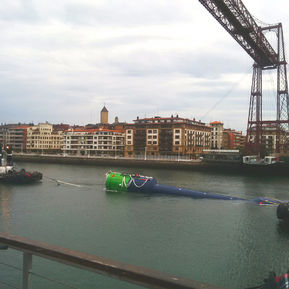
\includegraphics{/home/lewi/geaWaves/gea-waves/_hugo/content/tfg/1MEMORIA/imgMemoria/528-marmok-puente.jpg}
  \caption{}
  \end{figure}

  Figura 5.28: Fotografía del traslado de MARMOK-A-5,
  \href{https://www.tecnalia.com/es/energia-medioambiente/noticias/oceantec-instala-en-bimep-su-primer-dispositivo-para-el-aprovechamiento-de-la-energia-de-las-olas.htm}{Teclania\textgreater{}Noticias}

  El MARMOK-A-5 tiene la forma de una boya gigante y se trata de un
  primer dispositivo de baja potencia (30kW) de unas dimensiones de 5
  metros de diámetro, 42 metros de alto y un peso aproximado de 80
  toneladas.

  El principio de generación eléctrica se consigue gracias a que en el
  interior de la estructura central de la boya se crea una columna de
  agua, que con el movimiento desacompasado de las olas, ejerce de
  pistón, comprimiendo y descomprimiendo una cámara de aire que queda en
  el interior de la parte superior, siendo este flujo bidireccional
  aprovechado por unas turbinas que giran siempre en la misma dirección.

  A finales de 2017, el dispositivo
  \href{https://tidalenergytoday.com/2017/12/15/wave-device-at-bimep-marks-power-export-anniversary/}{cumplió}
  su primer año de implementación en bimep y gracias al proyecto europeo
  Opera, financiado con fondos públicos, se dispone de datos de
  funcionamiento en condiciones reales de mar, lo que permitirá diseñar
  un dispositivo pre-comercial de gran potencia, 300 kW. Paralelamente
  se está avanzando en el diseño del sistema de fondeo, el desarrollo de
  la electrónica de control y el diseño del sistema de extracción (PTO)
  incluidas las turbinas, información recogida en el
  \href{http://www.oceantecenergy.com/}{desarrollo tecnolóligo de
  Oceantec}.

  En marzo del 2018, el organismo de certificación de renovables
  \href{https://www.dnvgl.com/energy/generation/renewables-certification/index.html}{DNV
  GL} emitió la declaración de conformidad para el convertidor
  Marmok-A5, tras haber evaluado su diseño y sistema de amarre. Para
  lograr esta calificación, también se identificó el modelo de falla y
  clasificación de riesgos del convertidor. El convertidor se descompuso
  en sistemas, subsistemas y componentes, con la intención de considerar
  diferentes fases como, operación, fabricación, transporte e
  instalación; y así, lograr identificar tipos nuevos de fallo y
  acciones de mitigación, tal y como se establece en el proyecto OPERA.

  DNV GL, además de proporcionar el proceso de calificación de la
  tecnología, también está guiando en la aplicación de métodos de
  evaluación que permitan identificar de forma sistemática y priorizada
  novedades, incertidumbres y riesgos.

  El proyecto OPERA, coordinado por Tecnalia y 12 socios más entre
  académicos e industriales, {[}{[}realizó una evaluación inicial de la
  configuración base de Marmok-A5, seguida de un monitoreo periódico de
  datos para evaluar y actualizar los riesgos específicos. Además, este
  proyecto{]}{]} tiene como objetivo desarrollar y eliminar los riesgos
  de las tecnologías que operan para extraer la energía de las olas,
  reduciendo el coste de operación en un 50\% y, consecuentemente,
  acelerar el despliegue de energía marina renovable.

  \url{https://tidalenergytoday.com/2018/03/05/oceantecs-wave-energy-device-breaks-de-risking-ground/}
\item
  Pelamis, Galicia

  Estructura muy resistente, pensada para zonas con condiciones muy
  adversas. Se estima que 30 de estos sistemas podrían cubrir las
  necesidades energéticas de unos 20.000 hogares europeos,
  \href{https://www.solucionesintegralesendesa.com/blog/equipamiento-hogar/ahorro-hogar/energia-undimotriz-el-poder-de-las-olas/}{endesa
  2015}.

  Norvento experimenta con tecnología Pelamis, en un emplazamiento
  \emph{offshore} en las costas de Galicia,
  \href{http://www.interempresas.net/Energia/Articulos/126331-Generar-energia-a-partir-de-energia-undimotriz.html}{interempresas-Proyecto
  Fahemar}. Aunque, recientemente su actividad, se ha centrado en la
  energía eólica, su especialidad siendo la mayor empresa eólica de
  galicia. En abril de 2018, se anunció la construción del primer parque
  experimental de I+D+i en España vinculado a la energía eólica,
  \href{http://www.economiaengalicia.com/articulo/empresa/norvento-construira-primer-parque-experimental-idi-espana-vinculado-energia-eolica/20170404180131003321.html}{economia-en-galicia}.

  ¿¿¿¿Narvantia es Norvanto? han hecho o no algun parque eólico en el
  océano?
  \url{http://renews.biz/110374/navantia-dispatches-ea1-jackets/}
\item
  Prototipo (J+B) 2B, Galicia

  El promotor Galicia Mar Renovables (La Coruña) fue fundada con el
  objeto de construir, instalar, comprobar el funcionamiento y explotar
  el sistema (J+B) 2B, para producir energía electrica a partir de las
  olas del mar, cuya boya preserie está fondeada en la Ría de Ares (La
  Coruña).
  \href{http://www.interempresas.net/Energia/Articulos/126331-Generar-energia-a-partir-de-energia-undimotriz.html}{interempresas-Proyecto
  Fahemar}

  En enero de 2017, se publicó que la nave de Galicia Mar Renovables
  podría pasar a la Xunta al no haber comprador; construcción finalizada
  en 2013 pero que nunca tuvo actividad. Ni en la subasta del 16 de
  junio, con una valoración de salida de 889.651,50 euros, ni en el
  proceso de adjudicación directa abierto ese mismo día, sin un precio
  mínimo de venta establecido.
  \href{https://www.lavozdegalicia.es/noticia/ferrol/carino/2017/01/19/nave-galicia-mar-carino-pasar-xunta-haber-comprador/0003_201701F19C7994.htm}{La
  voz de Galicia, 19/01/2017}. Hoy en día, la empresa, con sede en
  Ferrol (A Coruña), aún está activa. Aunque, tanto en 2010 como en el
  2012 realizó cambios en su objeto social, ampliando su campo en
  actividades de investigación y consultoría en energías renovabes de
  las mareas, solar, y eólica,
  \href{https://www.infoempresa.com/es-es/es/empresa/galicia-mar-renovables-sl}{infoEmpresas}.
\item
  Pipo System, Galicia

  El Consorcio de Portos de Galicia, Sogama, Cetmar, Inega e Igape, está
  ensayando su prototipo en un emplazamiento offshore y con tecnología
  Pipo System, el sistema \textbf{APC-Pisys} consta de dos boyas (una en
  superficie y otra sumergida de volumen variable que transmiten su
  movimiento lineal y lo convierte en rotativos, que finalmente son
  convertidos a una sola dirección. Las boyas siempre se mueven en
  direcciones opuestas, incrementando sus fuerzas y carreras
  simultáneas. Una tercera boya mantiene una profundidad constante
  mediante sus amarres al fondo marino. En esta boya de posicionamiento,
  están alojados los sistemas de control, generación y medición de la
  potencia. Los sistemas de medición oceanográficos disponen de un
  habitáculo ubicado en el interior de la boya de superficie y de
  soportes específicos externos.
  \href{http://www.interempresas.net/Energia/Articulos/126331-Generar-energia-a-partir-de-energia-undimotriz.html}{interempresas-Proyecto
  Fahemar}

  La empresa patentó a nivel mundial el sistema, contó con el apoyo
  financiero del Ministerio de Economía y Competitividad y la Comunidad
  Europea (Fondos Feder), y su desarrollo se traduce en diez años de
  trabajo, 14 millones de inversión y la colaboración de importantes
  centros científicos como es el caso de la Plataforma Oceánica de
  Canarias y las universidades de Zaragoza y Politécnica de Cataluña.
  \href{http://www.laprovincia.es/sociedad/2012/10/21/carrera-boya-inteligente/491794.html}{Diario
  de Las Palmas}

  A una escala 1:5 y mediante un oleaje intermedio como el que se da en
  las Islas Canarias (Boyas Las Palmas I y II de Puertos del Estado), el
  sistema APC-PISYS, puede alcanzar potencias de entre 100 y 150 Kw.

  En 2012 durante las maniobras de amarre no se previó unas corrientes
  que llevaron la boya a la deriva, pero se recuperó sin problema y
  quedó listo para su comercialización. Para ello cuentan con el apoyo
  del Ministerio de Economía, y precisan de una gran empresa que ponga
  el capital para crear la industria para la fabricación,
  previsiblemente en Canarias.

  Desde entonces no hay constancia de que se esté comercializando
  energía obtenida mediante este dispositivo, así mismo la página
  oficial de Pipo System ya no está operativa,
  \href{https://web.archive.org/web/20170427103046/http://www.piposystems.com/welcome.html}{WayBackMachine,
  piposystem}.
\item
  Proyecto "Wavenergy", Santa Cruz de Tenerife (Canarias)

  La Unión Europea (EU) aprobó este proyecto concebido para generar
  energía con el impacto de las olas en el muelle del futuro puerto de
  Granadilla (Tenerife), iniciativa en la que la Autoridad Portuaria de
  Santa Cruz de Tenerife es uno de los socios que, junto con el Cabildo
  de Tenerife, INGEMAR, ITER, EIGSI y WAVEGEN desarrollará el citado
  proyecto. El proyecto contará con un presupuesto total de 400.000
  euros, y ha sido aprobado por Bruselas en la convocatoria 2006 de
  ayudas del Fondo Europeo de Desarrollo Regional (FEDER),
  correspondiente al ``Espacio Atlántico-Interreg IIIB''. Su redacción
  fue coordinada por la Oficina de Representación del Cabildo ante el
  Estado y la UE, junto con técnicos de las entidades participantes,
  durante los tres meses que duraron los trabajos para su elaboración.
  Asimismo, en un hecho insólito en este tipo de convocatorias, la Unión
  Europea ha concedido el 91,4\% de la subvención total a la que se
  aspiraba.
  \href{http://www.mapama.gob.es/ministerio/pags/Biblioteca/Revistas/pdf_AM\%2FAM_2008_83_26_31\%5B1\%5D.pdf}{Proyecto
  santoña, dic 2008}
\item
  En Sant Feliu (Girona)

  Abencis Seapower está promoviendo un captador puntual onshore,
  consistente en una boya que mediante un brazo rígido a modo de
  palanca, transmite la energía de la ola a un árbol rotativo que mueve
  el rotor del generador.
\item
  En Madrid y promovido por un consorcio formado por Cedex, Elytt y
  Neures TEC se está desarrollando el proyecto Undigen, cuyo objetivo es
  el diseño de un generador Wedge, lineal de alta reluctancia, para su
  posterior aplicación a dispositivos de olas.
  \href{http://www.interempresas.net/Energia/Articulos/126331-Generar-energia-a-partir-de-energia-undimotriz.html}{interempresas-Proyecto
  Fahemar}
\end{itemize}
